\chapter{Features' importance}

After having determined the most performant algorithm, which is Random Forest, it is time to go further and analyse which features impact the results of classification the most. In order to do that, six tools will be examined: Lime \cite{lime}, ELI5 \cite{mikhail_korobov_eli5_nodate}, YellowBrick \cite{bengfort_yellowbrick_2018}, Treeinterpreter \cite{ando_saabas_treeinterpreter_nodate}, dtreeviz \cite{terence_parr_dtreeviz_nodate} and export\_graphviz tool from scikit-learn, where the last three ones are designed for Decison Tree classifiers, but can also work with unitary trees from the Random Forest.

However, before going deeper into features' importance classification, the features itself should be discussed. The power system presented \cite{adhikari_power_2014} is described by 128 features: 116 provided by four phasor measurement units\footnote{Phasor measurement units measure the electrical waves on an electricity grid} (each one provides 29 types of measurements) and 12 other features are reserved for control panel logs, snort alerts, relay logs of 4 phasors. The mentioned 116 features, each has a label formed by concatenation of the source phasor reference (it can be R1, R2, R3, R4) and the measurement name, as provided in table \ref{tab:pmu_mes}.

\begin{table}[H]
    \centering
    \caption[Phasor measurements]{Phasor measurements \cite{adhikari_power_2014}} \label{tab:pmu_mes}
    \begin{tabular}{|c|c|}\hline
        \textbf{Feature}&\textbf{Description} \\\hline
        PA1:VH – PA3:VH&Phase A - C Voltage Phase Angle \\\hline
        PM1: V – PM3: V&Phase A - C Voltage Phase Magnitude \\\hline
        PA4:IH – PA6:IH&Phase A - C Current Phase Angle \\\hline
        PM4: I – PM6: I&Phase A - C Current Phase Magnitude \\\hline
        PA7:VH – PA9:VH&Pos. – Neg. – Zero Voltage Phase Angle \\\hline
        PM7: V – PM9: V&Pos. – Neg. – Zero Voltage Phase Magnitude \\\hline
        PA10:VH - PA12:VH&Pos. – Neg. – Zero Current Phase Angle \\\hline
        PM10: V - PM12: V&Pos. – Neg. – Zero Current Phase Magnitude \\\hline
        F&Frequency for relays \\\hline
        DF&Frequency Delta (dF/dt) for relays \\\hline
        PA:Z&Appearance Impedance for relays \\\hline
        PA:ZH&Appearance Impedance Angle for relays \\\hline
        S&Status Flag for relays \\\hline
    \end{tabular}
\end{table}

\section{Lime}
Lime is a tool that is used to explain the behaviour of machine learning classifiers. It supports, as for this day, only the explanation of individual predictions. As output it gives a list of features ordered by their relative importance in the prediction of this particular sample.

In order to class the features according to their importance, Lime approximates the model by an interpretable one, created based on perturbing the features of the examined instance. More the perturbed instances are similar to the examined instance, higher is the weight that gets the perturbed feature.

Since in this case the explanations of single samples are not really interesting, an attempt to generalize the results was made: Lime explainer was run on 100 false predictions of a chosen class. The results are concatenated together, and for all the features that are duplicated, the importance is calculated as the mean value of the importances and only one entry is kept with the calculated average importance. This algorithm was also run omitting the differentiation between classes. The results, reduced to 10 entries each, are shown below.

For NoEvents class:
\begin{verbatim}
                                     importance
 feature                                      
 R2-PM1:V > 130872.03                -0.013013
 R3-PA2:VH <= -93.75                 -0.011134
 R2-PA7:VH <= -101.20                -0.010218
 R3-PM2:V > 130431.15                -0.009583
 R2-PM7:V > 130857.40                -0.009377
 ...                                       ...
 R3-PM5:I <= 330.70                   0.005762
 0.00 < R1-PA12:IH <= 32.04           0.007514
 128762.21 < R2-PM1:V <= 129859.49    0.007776
 R3-PM2:V <= 128425.29                0.007998
 R4-PA5:IH > 115.38                   0.008534
 
 [361 rows x 1 columns]
\end{verbatim}

For Attack class:
\begin{verbatim}
                                   importance
    feature                                 
    R3-PA2:VH > 113.97             -0.012837
    -97.10 < R4-PA7:VH <= -35.66   -0.010994
    -97.43 < R1-PA7:VH <= -35.85   -0.010306
    R2-PA2:VH > 114.00             -0.009730
    R3-PM2:V <= 128425.29          -0.006914
    ...                                  ...
    R3-PA2:VH <= -93.75             0.008307
    R3-PA7:VH <= -101.22            0.008676
    R2-PM1:V > 130872.03            0.009242
    R3:S > 0.00                     0.010717
    R2-PA7:VH <= -101.20            0.014018
    
    [380 rows x 1 columns]
\end{verbatim}

For Natural class: 
\begin{verbatim}
                            importance
    feature                          
    R2-PA5:IH <= -74.26     -0.003613
    R4-PM3:V > 132484.78    -0.002835
    R4-PM2:V > 132187.18    -0.002437
    R2-PM7:V <= 128751.24   -0.002290
    R2-PM1:V <= 128762.21   -0.002151
    ...                           ...
    R1-PA1:VH > 71.28        0.003518
    R2-PM7:V > 130857.40     0.003693
    R2-PA5:IH > 63.30        0.004103
    R3:F > 60.00             0.004873
    R2:F > 60.00             0.005168
    
    [331 rows x 1 columns]]
\end{verbatim}

For all classes:
\begin{verbatim}
                                 importance
    feature                                
    R3-PM2:V <= 128425.29         -0.006715
    R2-PA7:VH > 65.91             -0.006353
    R3-PM5:I <= 330.70            -0.006009
    -40.44 < R3-PA1:VH <= 65.76   -0.005808
    R3-PA4:IH <= -65.22           -0.005764
    ...                                 ...
    R2-PA3:VH <= -75.28            0.005588
    R3-PA4:IH > 102.49             0.005723
    R4-PA1:VH > 71.50              0.007481
    R3-PM2:V > 130431.15           0.008501
    R2-PM1:V > 130872.03           0.009070
    
    [331 rows x 1 columns]
\end{verbatim}
\section{ELI5}

\section{YellowBrick}

\section{Random Forest and Decision Trees}
\subsection{Treeinterpreter}

\subsection{dtreeviz}


\begin{figure}[tb]
    \centering
    \makebox[\textwidth]{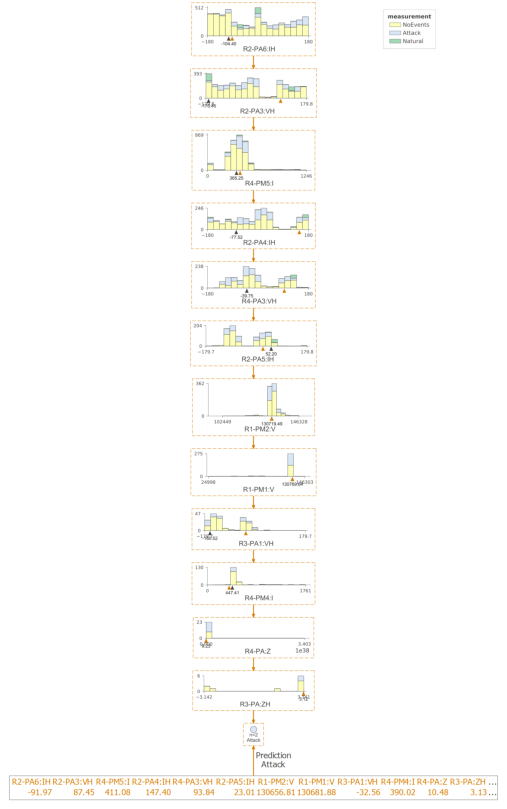
\includegraphics[width=.9\paperwidth, height=.9\textheight]{images/dtreeviz}}
    \caption{dtreeviz's visualisation of the prediction path for Natural event mispredicted as Attack}
    \label{fig:dtreeviz}
\end{figure}

\subsection{scikit-learn export\_graphviz}